\documentclass{beamer}
\usepackage{tikz}
\usepackage{listings}
\lstset{language=python,
                basicstyle=\footnotesize\ttfamily,
                keywordstyle=\footnotesize\color{black}\ttfamily,
}
\usetikzlibrary{calc,positioning,shadows.blur,decorations.pathreplacing}

%% arguments: x, y, width, height. it is measured from bottom left corner
\newcommand\tikzbox[5]{%
      \draw (#1, #2) -- +(0, #4) -- +(#3, #4) -- +(#3, 0) -- +(0, 0) node[align=left,right] at +(0,#4/2) {#5}
}

\newcommand\raidbox[5]{%
  \tikzbox{#1}{#2}{#3}{#4}{
    \normalsize\texttt{#5} \\
    \tiny\texttt{   backup} \\
    \tiny\texttt{   var/anonym} \\
    \tiny\texttt{   var/public} \\
    \tiny\texttt{   var/private}}
}
\renewcommand{\baselinestretch}{0.5}

\begin{document}
\begin{frame}{Old User Home}
    \frametitle{User Home}
    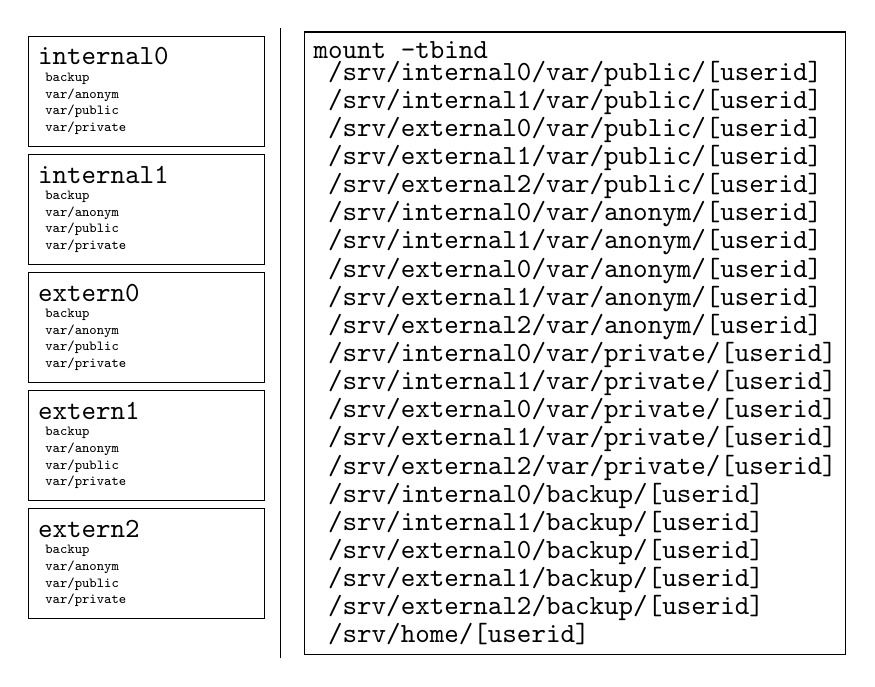
\begin{tikzpicture}
        % The Raids
        \raidbox{0}{1.5*4}{3}{1.4}{internal0};
        \raidbox{0}{1.5*3}{3}{1.4}{internal1};
        \raidbox{0}{1.5*2}{3}{1.4}{extern0};
        \raidbox{0}{1.5*1}{3}{1.4}{extern1};
        \raidbox{0}{1.5*0}{3}{1.4}{extern2};
        % Separation line
        \draw (3.2, -0.5) -- +(0, 1.4*5 + 1);

        % The old mammut
        \node[draw,align=left,right] at (3.5, 0.7*5) {
          \texttt{mount -tbind \ } \\
          \texttt{   /srv/internal0/var/public/[userid] \ }\\
          \texttt{   /srv/internal1/var/public/[userid] \ }\\
          \texttt{   /srv/external0/var/public/[userid] \ }\\
          \texttt{   /srv/external1/var/public/[userid] \ }\\
          \texttt{   /srv/external2/var/public/[userid] \ }\\
          \texttt{   /srv/internal0/var/anonym/[userid] \ }\\
          \texttt{   /srv/internal1/var/anonym/[userid] \ }\\
          \texttt{   /srv/external0/var/anonym/[userid] \ }\\
          \texttt{   /srv/external1/var/anonym/[userid] \ }\\
          \texttt{   /srv/external2/var/anonym/[userid] \ } \\
          \texttt{   /srv/internal0/var/private/[userid] \ }\\
          \texttt{   /srv/internal1/var/private/[userid] \ }\\
          \texttt{   /srv/external0/var/private/[userid] \ }\\
          \texttt{   /srv/external1/var/private/[userid] \ }\\
          \texttt{   /srv/external2/var/private/[userid] \ }\\
          \texttt{   /srv/internal0/backup/[userid] \ }\\
          \texttt{   /srv/internal1/backup/[userid] \ }\\
          \texttt{   /srv/external0/backup/[userid] \ }\\
          \texttt{   /srv/external1/backup/[userid] \ }\\
          \texttt{   /srv/external2/backup/[userid] \ }\\
          \texttt{   /srv/home/[userid]}};
    \end{tikzpicture}
\end{frame}

\begin{frame}{Public Listing}
    \frametitle{\texttt{/srv/public}}
    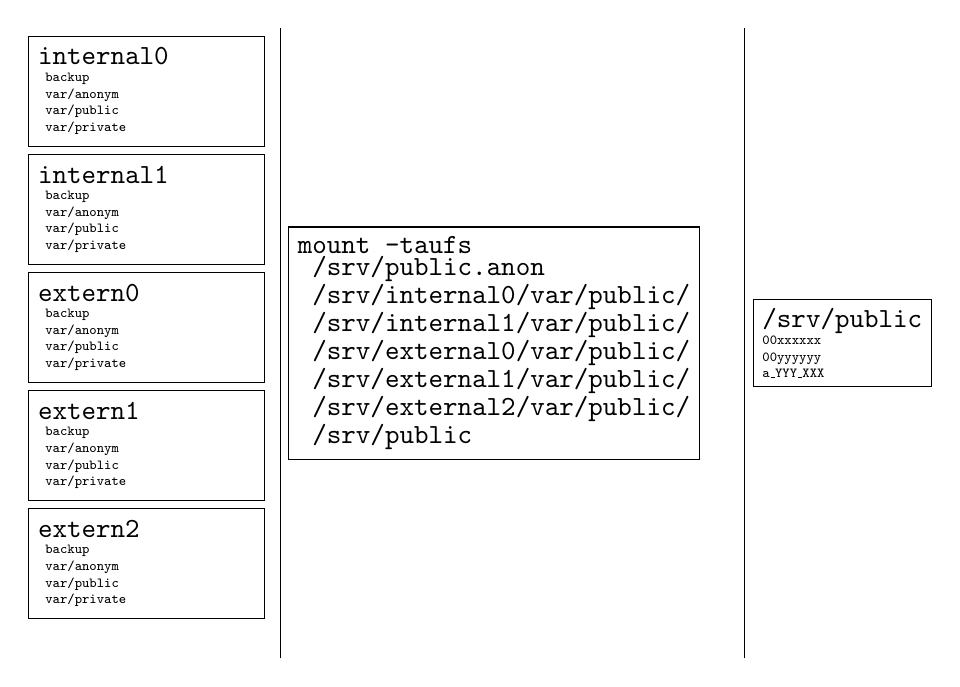
\begin{tikzpicture}
        % The Raids
        \raidbox{0}{1.5*4}{3}{1.4}{internal0};
        \raidbox{0}{1.5*3}{3}{1.4}{internal1};
        \raidbox{0}{1.5*2}{3}{1.4}{extern0};
        \raidbox{0}{1.5*1}{3}{1.4}{extern1};
        \raidbox{0}{1.5*0}{3}{1.4}{extern2};
        % Separation line
        \draw (3.2, -0.5) -- +(0, 1.4*5 + 1);
        
        % The old mammut
        \node[draw,align=left,right] at (3.3, 0.7*5) {
          \texttt{mount -taufs } \\
          \texttt{   /srv/public.anon }\\
          \texttt{   /srv/internal0/var/public/ }\\
          \texttt{   /srv/internal1/var/public/ }\\
          \texttt{   /srv/external0/var/public/ }\\
          \texttt{   /srv/external1/var/public/ }\\
          \texttt{   /srv/external2/var/public/ }\\
          \texttt{   /srv/public}};
        \draw (9.1, -0.5) -- +(0, 1.4*5 + 1);
        \node[draw,align=left,right] at (9.2, 0.7*5) {
          \texttt{/srv/public} \\
          \tiny\texttt{00xxxxxx} \\
          \tiny\texttt{00yyyyyy} \\
          \tiny\texttt{a\_YYY\_XXX}
        };
    \end{tikzpicture}
\end{frame}

\begin{frame}{Anon listing}
    \frametitle{\texttt{/srv/public.anon}}
    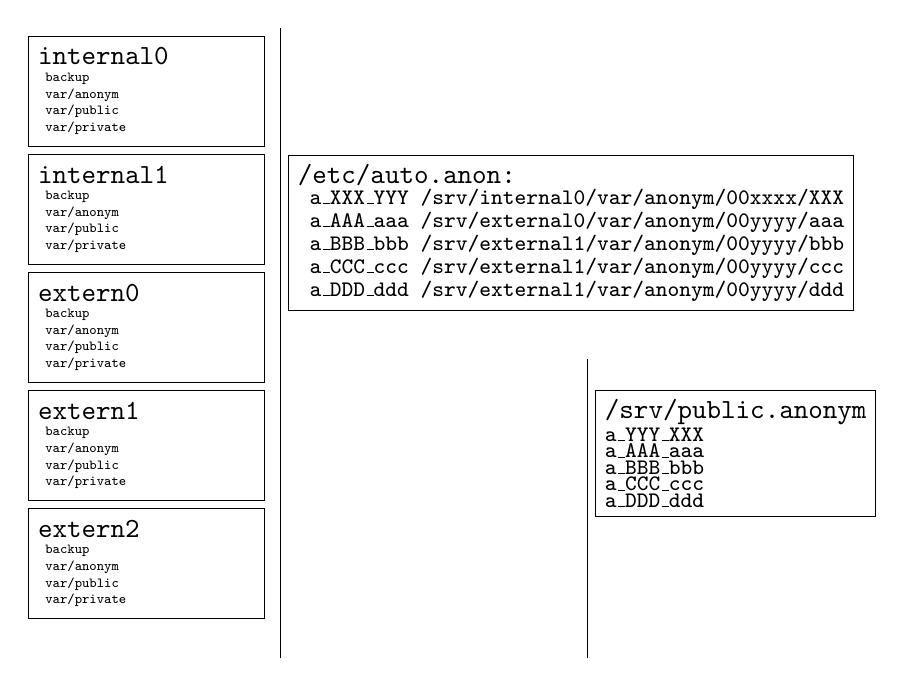
\begin{tikzpicture}
        % The Raids
        \raidbox{0}{1.5*4}{3}{1.4}{internal0};
        \raidbox{0}{1.5*3}{3}{1.4}{internal1};
        \raidbox{0}{1.5*2}{3}{1.4}{extern0};
        \raidbox{0}{1.5*1}{3}{1.4}{extern1};
        \raidbox{0}{1.5*0}{3}{1.4}{extern2};
        % Separation line
        \draw (3.2, -0.5) -- +(0, 1.4*5 + 1);
        
        % The old mammut
        \node[draw,align=left,right] at (3.3, 0.7*7) {
          \texttt{/etc/auto.anon:} \\
          \footnotesize\texttt{ a\_XXX\_YYY  /srv/internal0/var/anonym/00xxxx/XXX }\\
          \footnotesize\texttt{ a\_AAA\_aaa  /srv/external0/var/anonym/00yyyy/aaa }\\
          \footnotesize\texttt{ a\_BBB\_bbb  /srv/external1/var/anonym/00yyyy/bbb }\\
          \footnotesize\texttt{ a\_CCC\_ccc  /srv/external1/var/anonym/00yyyy/ccc }\\
          \footnotesize\texttt{ a\_DDD\_ddd  /srv/external1/var/anonym/00yyyy/ddd }};
        \draw (7.1, -0.5) -- +(0, 1.4*2 + 1);
        \node[draw,align=left,right] at (7.2, 0.7*3) {
          \texttt{/srv/public.anonym} \\
          \footnotesize\texttt{a\_YYY\_XXX}\\
          \footnotesize\texttt{a\_AAA\_aaa}\\
          \footnotesize\texttt{a\_BBB\_bbb}\\
          \footnotesize\texttt{a\_CCC\_ccc}\\
          \footnotesize\texttt{a\_DDD\_ddd}};
    \end{tikzpicture}
\end{frame}


\begin{frame}{Mammutfs user home}
%  LocalWords:  mountpoint
    \frametitle{Mammutfs: User Home}
    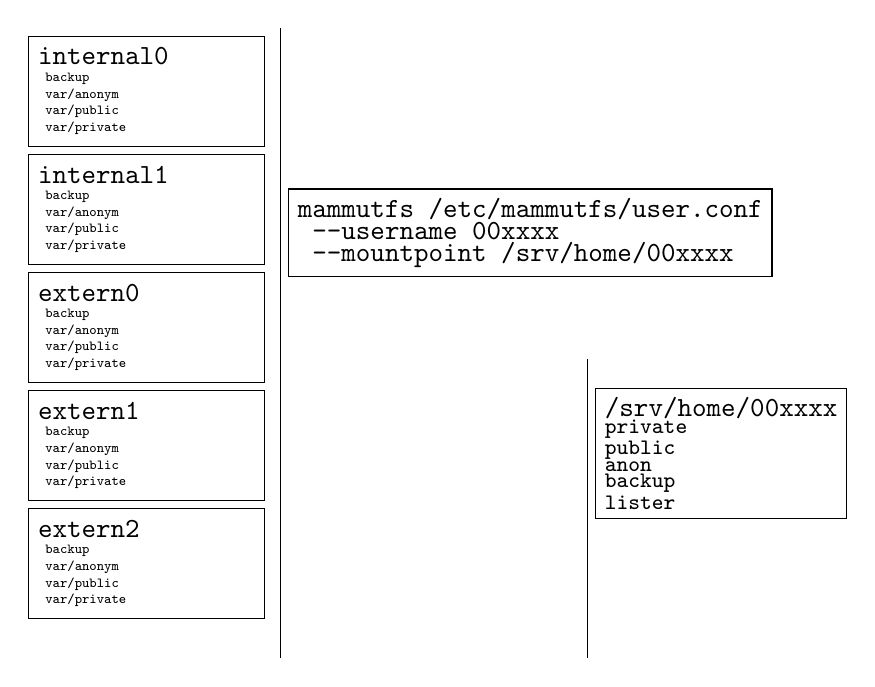
\begin{tikzpicture}
        % The Raids
        \raidbox{0}{1.5*4}{3}{1.4}{internal0};
        \raidbox{0}{1.5*3}{3}{1.4}{internal1};
        \raidbox{0}{1.5*2}{3}{1.4}{extern0};
        \raidbox{0}{1.5*1}{3}{1.4}{extern1};
        \raidbox{0}{1.5*0}{3}{1.4}{extern2};
        % Separation line
        \draw (3.2, -0.5) -- +(0, 1.4*5 + 1);

        % The new shit
        \node[draw,align=left,right] at (3.3, 0.7*7) {
          \texttt{mammutfs /etc/mammutfs/user.conf }\\
          \texttt{  --username 00xxxx }\\
          \texttt{  --mountpoint /srv/home/00xxxx}};
        \draw (7.1, -0.5) -- +(0, 1.4*2 + 1);
        \node[draw,align=left,right] at (7.2, 0.7*3) {
          \texttt{/srv/home/00xxxx} \\
          \footnotesize\texttt{private}\\

          \footnotesize\texttt{public}\\
          \footnotesize\texttt{anon}\\
          \footnotesize\texttt{backup}\\
          \footnotesize\texttt{lister}
        };
    \end{tikzpicture}
\end{frame}

\begin{frame}{Mammutfs: Modules}
    \frametitle{Mammutfs: Modules}
    \begin{tikzpicture}
        % The Raids
        \tikzbox{0}{1.1}{3}{6.5}{};
        \node[align=left,right] at (0,4) {
          Default: \\
          The users\\
          home directory\\
         % \texttt{$\backslash$}\\
          \begin{itemize}
          \item List active modules
          \item Read only
          \item Purely virtual
          \end{itemize}
        };
        \tikzbox{3.3}{1.1*6}{2}{1}{anon\\\texttt{$\backslash$anon}}
        	node[right] at +(2, 0.5) {\small Anonymous upload: filters for DIR, notifies};
        \tikzbox{3.3}{1.1*5}{2}{1}{public\\\texttt{$\backslash$public}}
        	node[right] at +(2, 0.5) {\small Public upload: notifies};
        \tikzbox{3.3}{1.1*4}{2}{1}{private\\\texttt{$\backslash$private}}
        	node[right] at +(2, 0.5) {\small Private upload: nothing special};
        \tikzbox{3.3}{1.1*3}{2}{1}{backup\\\texttt{$\backslash$backup}}
        	node[right] at +(2, 0.5) {\small Backup upload: nothing special};
        \tikzbox{3.3}{1.1*2}{2}{1}{lister\\\texttt{$\backslash$lister}}
        	node[right] at +(2, 0.5) {\small Public file listing: R/O, all files};
        \tikzbox{3.3}{1.1*1}{2}{1}{***\\\texttt{$\backslash$???}}
        	node[right] at +(2, 0.5) {\small More modules};
        % Separation line
        \draw (3.2, 1.1) -- +(0, 1.1*5 + 1);

    \end{tikzpicture}
\end{frame}
% TODO Add /etc/mammutfs/user.conf


\begin{frame}{Mammutfs Anon Directories}
    \frametitle{Mammutfs: Public folder}
    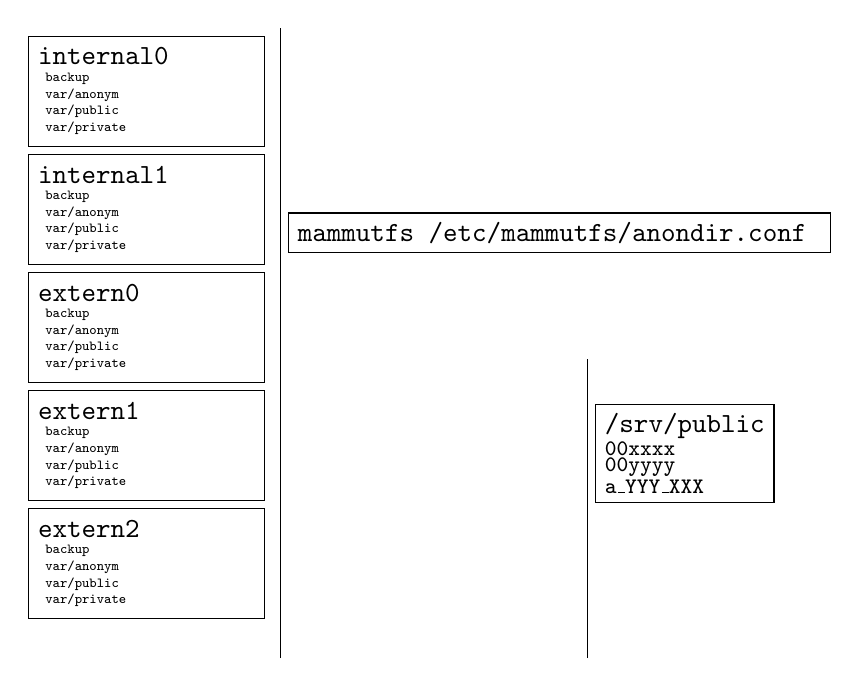
\begin{tikzpicture}
        % The Raids
        \raidbox{0}{1.5*4}{3}{1.4}{internal0};
        \raidbox{0}{1.5*3}{3}{1.4}{internal1};
        \raidbox{0}{1.5*2}{3}{1.4}{extern0};
        \raidbox{0}{1.5*1}{3}{1.4}{extern1};
        \raidbox{0}{1.5*0}{3}{1.4}{extern2};
        % Separation line
        \draw (3.2, -0.5) -- +(0, 1.4*5 + 1);

        % The old mammut
        \node[draw,align=left,right] at (3.3, 0.7*7) {
          \texttt{mammutfs /etc/mammutfs/anondir.conf }};
        \draw (7.1, -0.5) -- +(0, 1.4*2 + 1);
        \node[draw,align=left,right] at (7.2, 0.7*3) {
          \texttt{/srv/public} \\
          \footnotesize\texttt{00xxxx} \\
          \footnotesize\texttt{00yyyy} \\
          \footnotesize\texttt{a\_YYY\_XXX}
        };
    \end{tikzpicture}
\end{frame}

\begin{frame}[fragile]
    \frametitle{Mammutfs: Management Socket}

    \begin{lstlisting}
/run/mammutfs_sockets
   nobody - The anon listing socket
   00xxxx - Running mammutfs for user 00xxxx
   00yyyy - Running mammutfs for user 00yyyy
 \end{lstlisting}
 
    \vspace{1cm}

    \begin{lstlisting}
tools/socket.py /run/mammutfs_sockets/00xxxx
$ HELP
FORCE-RELOAD
HELP
CLEARCACHE
$
{"op":"create",
  "path":"/srv/extern1/var/public/00xxxx/test"}
{"op":"modify",
  "path":"/srv/extern1/var/public/00xxxx/modify"}
{"op":"rename",
  "path":"/srv/extern1/var/public/00xxxx/old
  ->/srv/extern1/var/public/00xxxx/new"}
    \end{lstlisting}
\end{frame}
%  LocalWords:  extern  srv mammutfs
\end{document}
